\documentclass[12pt]{article}  

\usepackage
[colorlinks=true, pdfstartview=FitV, linkcolor=blue, citecolor=blue, urlcolor=blue]
{hyperref}

\usepackage{amssymb}  
\usepackage{amsthm}
\usepackage{amsmath}
\usepackage{graphics} 
\usepackage{graphicx} 
%\usepackage[latin1]{inputenc}
\usepackage{tikz}
\usepackage{pgfplots}
\usepackage{wrapfig}
\usepackage{caption}
\usepgfplotslibrary{polar}
\usepackage{ skull }
\usetikzlibrary{decorations.fractals}


% GNUPLOT required
\usepackage{verbatim}

\linespread{1.3}

%\addtolength{\textwidth}{80pt}
\addtolength{\evensidemargin}{20pt}
\addtolength{\oddsidemargin}{20pt}

%%%%%%%%%%%%%%%%%%%%%%%%%%%%%%%%%%%%%%%%%%%%%%
%  Begin user defined commands

\newcommand{\map}[1]{\xrightarrow{#1}}

\newcommand{\N}{\mathbb N}
\newcommand{\Z}{\mathbb Z}
\newcommand{\Primes}{\mathbb P}
\newcommand{\Q}{\mathbb Q}
\newcommand{\R}{\mathbb R}
\newcommand{\C}{\mathbb C}
\newcommand{\bz}{\mathbb Z}
\newcommand{\bq}{\mathbb Q}
\newcommand{\br}{\mathbb R}
\newcommand{\bc}{\mathbb C}
\newcommand{\al}{\alpha}
\newcommand{\be}{\beta}
\newcommand{\ga}{\gamma}
\newcommand{\de}{\delta}
\newcommand{\ep}{\epsilon}
\DeclareMathOperator{\lub}{l.u.b.}
%  End user defined commands
%%%%%%%%%%%%%%%%%%%%%%%%%%%%%%%%%%%%%%%%%%%%%%


%%%%%%%%%%%%%%%%%%%%%%%%%%%%%%%%%%%%%%%%%%%%%%
% These establish different environments for stating Theorems, Lemmas, Remarks, etc.

\newtheorem{Thm}{Theorem}
\newtheorem{Prop}[Thm]{Proposition}
\newtheorem{Lem}[Thm]{Lemma}
\newtheorem{Cor}[Thm]{Corollary}

\theoremstyle{definition}
\newtheorem{Def}[Thm]{Definition}

\theoremstyle{remark}
\newtheorem{Rem}[Thm]{Remark}
\newtheorem{Ex}[Thm]{Example}

\theoremstyle{definition}
\newtheorem{Exercise}{Problem}

\newenvironment{Solution}{\noindent\textbf{Solution.}}{}

%\renewcommand{\labelenumi}{(\alph{enumi})}
\renewcommand\qedsymbol{QED}
% End environments 
%%%%%%%%%%%%%%%%%%%%%%%%%%%%%%%%%%%%%%%%%%%%%%%
%Some commands to save paper


\setlength{\parindent}{0in}
\setlength{\parskip}{8pt}

\DeclareMathOperator{\arcsec}{arcsec}
\DeclareMathOperator{\arccot}{arccot}
\DeclareMathOperator{\arccsc}{arccsc}
\DeclareMathOperator{\LH}{\ \underset{\text{LH}}{=}\ }
\newcommand{\Dep}{\Delta_+}
\newcommand{\Dem}{\Delta_-}
\newcommand{\bu}{\mathbf u}
\newcommand{\bv}{\mathbf v}
\newcommand{\bw}{\mathbf w}
\newcommand{\bx}{\mathbf x}

\newcommand{\ora}{\overrightarrow}



\addtolength{\textwidth}{80pt}
\addtolength{\evensidemargin}{-40pt}
\addtolength{\oddsidemargin}{-40pt}
\addtolength{\topmargin}{-80pt}
\addtolength{\textheight}{1.8in}

\setlength{\parindent}{0in}
\setlength{\parskip}{8pt}

\DeclareMathOperator{\arcsinh}{arcsinh}

%%%%%%%%%%%%%%%%%%%%%%%%%%%%%%%%%%%%%%%%%%%%%%
% Now we're ready to start
%%%%%%%%%%%%%%%%%%%%%%%%%%%%%%%%%%%%%%%%%%%%%%

\begin{document}  

%\author{Your Name}
{\bf MATH 1103 Homework 8}\\
{\bf Due Wednesday March 28, 2018}

%Practice Problems (not to be turned in)

%{\bf Practice 1.\ } 
%{\bf Practice 2.\ } 
%{\bf Practice 3.\ } 
%{\bf Practice 4.\ }   \rule{\textwidth}{1pt}
%The homework to be turned in may be found on the next page.




{\bf Homework 8 problems to be turned in.}

{\bf 1.\ } Compute the following integrals as power series.

a)\ \[\int_0^1 \arctan x\ dx\]
b)\ \[\int_0^1\ \frac{\sin x}{x}\ dx\]
c)\ \[\int_0^x \exp(-t^2)\ dt\]

\begin{Solution}
a)\ Since 
\[\arctan x=x-\frac{x^3}{3}+\frac{x^5}{5}-\cdots=
\sum_{k=1}^\infty(-1)^{k-1}\frac{x^{2k-1}}{2k-1},
\]
we have
\[\begin{split}
\int_0^1 \arctan x\ dx
&=\int_0^1\sum_{k=1}^\infty(-1)^{k-1}\frac{x^{2k-1}}{2k-1}
=\sum_{k=1}^\infty(-1)^{k-1}\int_0^1\frac{x^{2k-1}}{2k-1}
=\sum_{k=1}^\infty\frac{(-1)^{k-1}}{(2k-1)(2k)}\\
&=\frac{1}{1\cdot 2}-\frac{1}{3\cdot 4}+\frac{1}{5\cdot 6}-\frac{1}{7\cdot 8}+\cdots
\end{split}
\]
b)\ Since 
\[\sin x=\sum_{k=0}^\infty(-1)^{k}\frac{x^{2k+1}}{(2k+1)!},
\quad\text{we have}\quad
\frac{\sin x}{x}=\sum_{k=0}^\infty(-1)^{k}\frac{x^{2k}}{(2k+1)!},
\]
so 
\[\int_0^1\frac{\sin x}{x}=\sum_{k=0}^\infty(-1)^{k}\frac{1}{(2k+1)(2k+1)!}
=\frac{1}{1\cdot 1!}-\frac{1}{3\cdot 3!}+\frac{1}{5\cdot 5!}-\cdots.
\]

c)\ Since 
\[\exp(x)=\sum_{k=0}^\infty \frac{x^k}{k!},\quad\text{we have}\quad
\exp(-t^2)=\sum_{k=0}^\infty \frac{(-t^2)^k}{k!}=\sum_{k=0}^\infty (-1)^k\frac{t^{2k}}{k!},\]
so
\[\int_0^x\exp(-t^2)\ dt=\sum_{k=0}^\infty (-1)^k\frac{x^{2k+1}}{(2k+1)k!}
=x-\frac{x^{3}}{3\cdot 1!}+\frac{x^{5}}{5\cdot 2!}-\frac{x^{7}}{7\cdot 3!}+\cdots.
\]
\end{Solution}

{\bf 2.\ } Let $a$ be a number between $0$ and $1$. 
Compute the area inside a unit circle with $y>0$ and $0\leq x\leq a$, as a power series in $a$. You will need the Binomial Series, see the table in chapter six. Express the coefficients in your series in terms of the numbers $P_k$, given by 

\[P_k=\frac{1\cdot 3\cdot 5\cdots(2k-1)}{2\cdot 4\cdot 6\ \ \ \ \cdots\ (2k)}.\]

\begin{center}
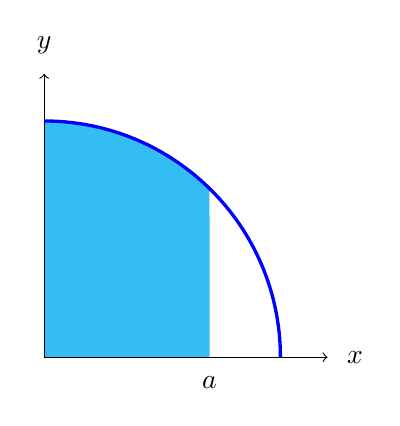
\begin{tikzpicture}[samples=25, domain=0:1.1, scale=3,
declare function = {f(\x) =sqrt(1-\x*\x);}]]
\fill[cyan!80] (0,0) -- plot [domain=0:0.7 ] (\x,{f(\x)}) --(0.7,0) -- cycle;
\draw[->] (0,0) -- (1.2,0);
\node[label=right: {$x$}] at (1.2,0) {};
\draw[->] (0,0) -- (0,1.2);
\node[label=above: {$y$}] at (0,1.2) {};
\node[label=below: {$a$}] at (0.7,0) {};
%\draw[blue, very thick] plot [domain=0:1 ] (\x,{f(\x)}) ;
\draw[blue, very thick] (1,0) arc (0:90:1);
\end{tikzpicture}
\end{center}

\begin{Solution} The area is given by the integral $\displaystyle{\int_0^a\sqrt{1-x^2}}$, 
to compute this as a power series in $a$. We start with the binomial series
\[
\sqrt{1+x}=1+\sum_{k=1}^\infty\binom{1/2}{k} x^k.
\]
Now 
\[\binom{1/2}{k}=\frac{\left(\frac{1}{2}\right)\left(\frac{1}{2}-1\right)
\left(\frac{1}{2}-2\right)\cdots\left(\frac{1}{2}-k+1\right)}
{k!}=
(-1)^{k-1}\frac{1\cdot 3\cdot 5\cdots (2k-3)}{2\cdot 4\cdot 6\cdots (2k)}=
(-1)^{k-1}\frac{P_k}{2k-1},
\]
so 
\[\sqrt{1+x}=1+\sum_{k=1}^\infty(-1)^{k-1}\frac{P_k}{2k-1} x^k,\]
and 
\[\sqrt{1-x^2}=1+\sum_{k=1}^\infty(-1)^{k-1}\frac{P_k}{2k-1} (-x^2)^k
=1-\sum_{k=1}^\infty\frac{P_k}{2k-1} x^{2k}.
\]
Now we integrate term-by-term: 
\[\int_0^a\sqrt{1-x^2}
=a-\sum_{k=1}^\infty\frac{P_k}{2k-1} \frac{a^{2k+1}}{2k+1}=
a-\sum_{k=1}^\infty \frac{P_k}{4k^2-1} a^{2k+1}.
\]
Comment: the subtraction removes the part the rectangle above the circle. 
\begin{center}
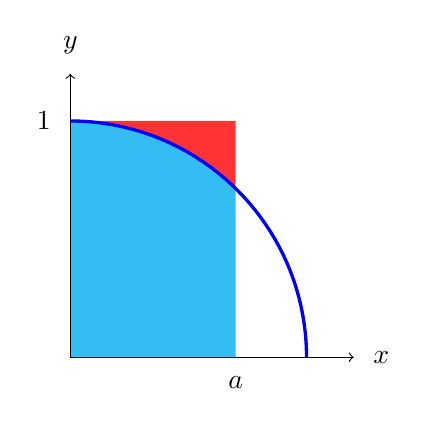
\begin{tikzpicture}[samples=25, domain=0:1.1, scale=3,
declare function = {f(\x) =sqrt(1-\x*\x);}]]
\fill[cyan!80] (0,0) -- plot [domain=0:0.7 ] (\x,{f(\x)}) --(0.7,0) -- cycle;
\fill[red!80] (0,1) --plot [domain=0:0.7 ] (\x,{f(\x)})  -- (0.7,1)--cycle;
\draw[->] (0,0) -- (1.2,0);
\node[label=right: {$x$}] at (1.2,0) {};
\draw[->] (0,0) -- (0,1.2);
\node[label=above: {$y$}] at (0,1.2) {};
\node[label=below: {$a$}] at (0.7,0) {};
\node[label=left: {$1$}] at (0,1) {};
%\draw[blue, very thick] plot [domain=0:1 ] (\x,{f(\x)}) ;
\draw[blue, very thick] (1,0) arc (0:90:1);
\end{tikzpicture}
\end{center}



\end{Solution}

\vskip10pt 
{\bf 3.\ } Recall that $\lfloor t\rfloor$ is the largest integer $\leq t$. Consider the function 
\[F(x)=\int_0^x\lfloor t\rfloor\ dt,\qquad 0\leq x\leq 4.\]
Give an explicit formula for $F(x)$ and draw the graph of $F(x)$ on the interval $[0,4]$. 
\newline
(Hint: Do not use upper and lower sums. Instead use a property of integrals and consider  successively $x$ in $[0,1]$, $[1,2]$, etc. Remember that in homework 7 you showed that $F(4)=6$.)
\begin{Solution}
For $0\leq x\leq 1$ we have $F(x)=\displaystyle{\int_0^x0}=0$.

For $1\leq x\leq 2$ we have $F(x)=\displaystyle{F(1)+\int_1^x 1}=0+x-1=x-1$.

For $2\leq x\leq 3$ we have $F(x)=\displaystyle{F(2)+\int_2^x 2}=1+2(x-2)=2x-3$.

For $3\leq x\leq 4$ we have $F(x)=\displaystyle{F(3)+\int_3^x 3}=3+3(x-3)=3x-6$.


\end{Solution}

\begin{center}
\begin{tikzpicture}[samples=25, domain=0:4.2, scale=.75]
\draw[->] (0,0) -- (4.2,0);
\node[label=right: {$x$}] at (4.2,0) {};
\draw[->] (0,0) -- (0,6.2);
\node[label=above: {$y$}] at (0,6.2) {};
\draw[blue, very thick] (0,0)--(1,0);
\draw[blue, very thick] (1,0)--(2,1);
\draw[blue, very thick] (2,1)--(3,3);
\draw[blue, very thick] (3,3)--(4,6);
\node[label=below: {$1$}] at (1,0) {};
\node[label=below: {$2$}] at (2,0) {};
\node[label=below: {$3$}] at (3,0) {};
\node[label=below: {$4$}] at (4,0) {};
\end{tikzpicture}
\end{center}

\end{document}








 
 
